\colorlet{chaptergrey}{gray}
\chapter[The relationship between black activity and simulated IFU kinematics in IllustrisTNG]{Misalignment and black hole activity}
\label{ch:halo_assembly}
\vspace{-5.25in}
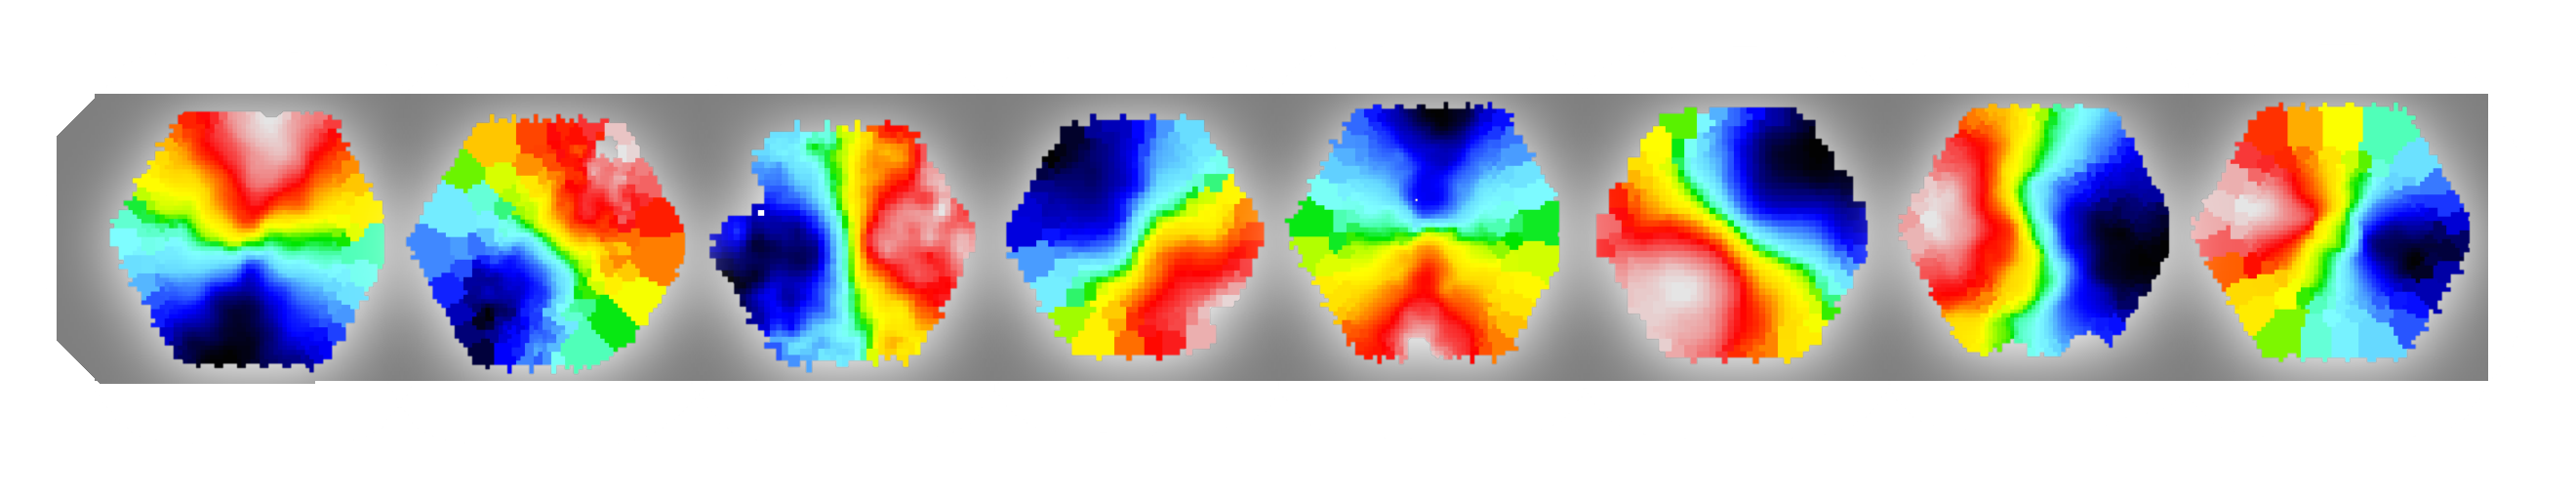
\includegraphics[height=1.39in]{thesis/latex/misalignment_intro/kin_mis_chapter_heading_grey.pdf}
\vspace{3in}

\epigraph{This chapter is based Duckworth, Starkenburg, Genel, Davis, Habouzit, Kraljic and Tojeiro (submitted). Here we investigate the temporal relationship between kinematically misaligned galaxies and black hole activity in IllustrisTNG.}

\section{Introduction}
Recent cosmological scale hydro-dynamical simulations have provided a clear insight into the relationship between the angular momentum of baryons and dark matter through cosmic time. A necessary component of realistic simulations is efficient feedback from both supermassive black holes (BH) and stars, required to, amongst other things, reproduce late type disks and solve the problem of catastrophic angular momentum loss \citep[e.g.][]{zavala2008, scannapieco2009}. Active galactic nuclei (AGN) and supernova explosions can also lead to dramatic redistribution of gas which regulate the angular momentum content of galaxies \citep[e.g.][]{genel2015, DeFelippis2017}.

`Quasar' (radiative) mode feedback releases huge amounts of energy through radiation from the accretion disk leading to high luminosity AGN and dramatic gas outflows \citep[e.g.][]{cattaneo2009, rubin2014, cheung2016}. Alternatively `radio' (kinetic) mode a term for lower luminosity AGN that host lower black hole accretion rates. In this instance energy is deposited into the surrounding gas via jets which drive outflows, heat the gas and suppress star formation \citep[][]{binney1995, ciotti2001, heckman2014}.

The relationship between AGN and kinematics has been the focus of several recent studies using data from Integral Field Spectroscopy. In particular, a potential new class of galaxy termed `red geyser' has been identified which host AGN and exhibit high velocity outflows in the spatial distribution of ionized gas \citep[][]{cheung2016, roy2018}. These outflows are often linked to a distinctive offset in rotation direction between the stars and gas. Detection of ongoing outflows is, however, rare ($\sim5-10$\% of the quiescent population). \citet{penny2018} demonstrate the importance of AGN feedback in low mass quiescent galaxies ($\mathrm{M_{stel} < 5 \times 10^{9}M_{\odot}}$). While the majority demonstrate no ionized gas present, quiescent galaxies (i.e. with reduced or null SFR) with an AGN show a clear decoupling in the rotation of stars and gas. However, the relationship of gas kinematics to BH feedback is not clear for all galaxies \citep[see also:][]{koudmani2019}. In particular, \citet{ilha2019} find that the typical decoupling between stars and gas for AGN defined galaxies are consistent with an inactive control sample. 

As introduced in \red{section X}, the decoupled rotation of stars and gas can be a natural result of external processes \cite[e.g.][]{davis2011, barrera2015, vdvoort2015, jin2016, bryant2019, duckworth2019_halo, li_decoupling2019}. Regardless of internal or external origin, kinematic misalignment in observations and simulations is linked with both a lower gas mass fraction and angular momentum as demonstrated in \red{section Y} \citep[see also;][]{starkenburg+19, khim2019}. In particular, \citet{starkenburg+19} highlight the importance of feedback leading to gas loss, enabling new or re-accretion as a mechanism for future misalignment in low mass galaxies. The question arises if misalignment is caused in the first instance by mergers or cosmic gas accretion (and hence making BH accretion easier) or if they are a result of AGN feedback leading to gas loss allowing for accretion of misaligned gas. The timescales of luminous AGN are typically much shorter than kinematic misalignment, making correlation at $z=0$ alone difficult. 

In this chapter, we study the temporal relationship between BH feedback, BH luminosity and kinematic misalignment in the cosmological scale hydrodynamical simulation of IllustrisTNG100 (hereafter referred to as TNG100). We use our sample of galaxies with mock MaNGA observations introduced in \red{section Z} to emulate what we may expect to see in IFS observations. In Section \ref{sec:methods_BH} we briefly introduce the specific methods associated with this work, before introducing results in Section \ref{sec:results_BH}. Finally we summarise the chapter in Section \ref{sec:summary_BH}.

\section{Methods} \label{sec:methods_BH}
As introduced in \S\ref{sec:sim_data_TNG}, we make use of data from the IllustrisTNG100 simulation. For studies of black hole properties, of particular relevance is the prescription of \citet{weinberger17} for BH feedback, which is modelled by two modes (quasar mode: high accretion, kinetic mode: low accretion). The transition threshold in terms of the Eddington ratio is 
\begin{equation}
\mathrm{f_{Edd}= \min ( 2x10^{-3}(M_{BH}/10^8 M_{\odot})^2 , 0.1)}
\end{equation}
so that BHs typically transition from quasar to kinetic mode around $\mathrm{M_{BH} = 10^{8}M_{\odot}}$. In the following, we separate our TNG100 galaxies by stellar mass at $\mathrm{M_{stel} = 10^{10.2}M_{\odot}}$ (nominally referred to low and high mass galaxies henceforth) which corresponds to this transition \citep[i.e. $\mathrm{M_{BH} \approx 10^{8}M_{\odot}}$, see Fig 1 in][]{li2019}. We do not explicitly follow the individual modes of accretion and feedback for each galaxy, which can alternate through its evolutionary history. Despite this, the transition threshold in TNG determines that we almost exclusively isolate the role of radiative feedback for our low mass sample. Our high mass sample, however, has been subject to both quasar and kinetic feedback over the last 8 Gyrs. To emulate what we may expect to see in IFS observations, we make use of our mock MaNGA sample as introduced in \S\ref{sec:mock_obs}.

\red{move to first introduction of following properties back in time?} The prior time evolution of BH and gas properties for each galaxy is followed by considering the main progenitor branch (most massive defined by stellar mass) in the sublink merger trees \citep{rgomez2015}. We compute BH bolometric luminosities as:
\begin{equation}
\mathrm{L_{bol, AGN}} = \frac{\varepsilon_r}{1 - \varepsilon_r} \dot{\mathrm{M}}_{\mathrm{BH}} \mathrm{c^2}
\end{equation}
where $\varepsilon_r=0.1$ is the radiative efficiency \citep[see discussion in][]{habouzit2019}, c the light speed, and $\dot{\mathrm{M}}_{\mathrm{BH}}$ the accretion rate onto the BH. Gas properties are defined within two effective radii ($\mathrm{R_{e}}$, radius containing half of the stellar mass within the galaxy), unless stated otherwise.

\section{Results} \label{sec:results_BH}
Each panel of Figure \ref{fig:overall_pop} shows the time evolution average of a property for all galaxies split by stellar mass at $\mathrm{M_{stel} = 10^{10.2}M_{\odot}}$, as explained in \S\ref{sec:methods_BH}. Splitting directly on BH mass at $\mathrm{M_{BH} = 10^{8}M_{\odot}}$ or enforcing stricter stellar mass cuts does not change any of our findings. We divide our sample by $\Delta$PA at $z=0$. For each sub-population, we find that the stellar mass distributions are consistent at $z=0$ for aligned and misaligned galaxies. Equivalent to our selection in \red{Section X}, we also split on specific star formation rate using the distance from the star-forming sequence (SFS) as defined in \citet{pillepich2019}. We select star forming ($\Delta \mathrm{log_{10}(SFR) > -0.5}$) and quenched galaxies ($\Delta \mathrm{log_{10}(SFR) \leq -1.0}$) at $z=0$. For clarity, the correlations with each misaligned sub-population in Figure \ref{fig:overall_pop} are summarized by Table \ref{tab:truth}. Additional time evolution properties can be found in Figure \ref{fig:overall_pop_additional}, and are also summarized in Table \ref{tab:truth}.

\begin{figure}
	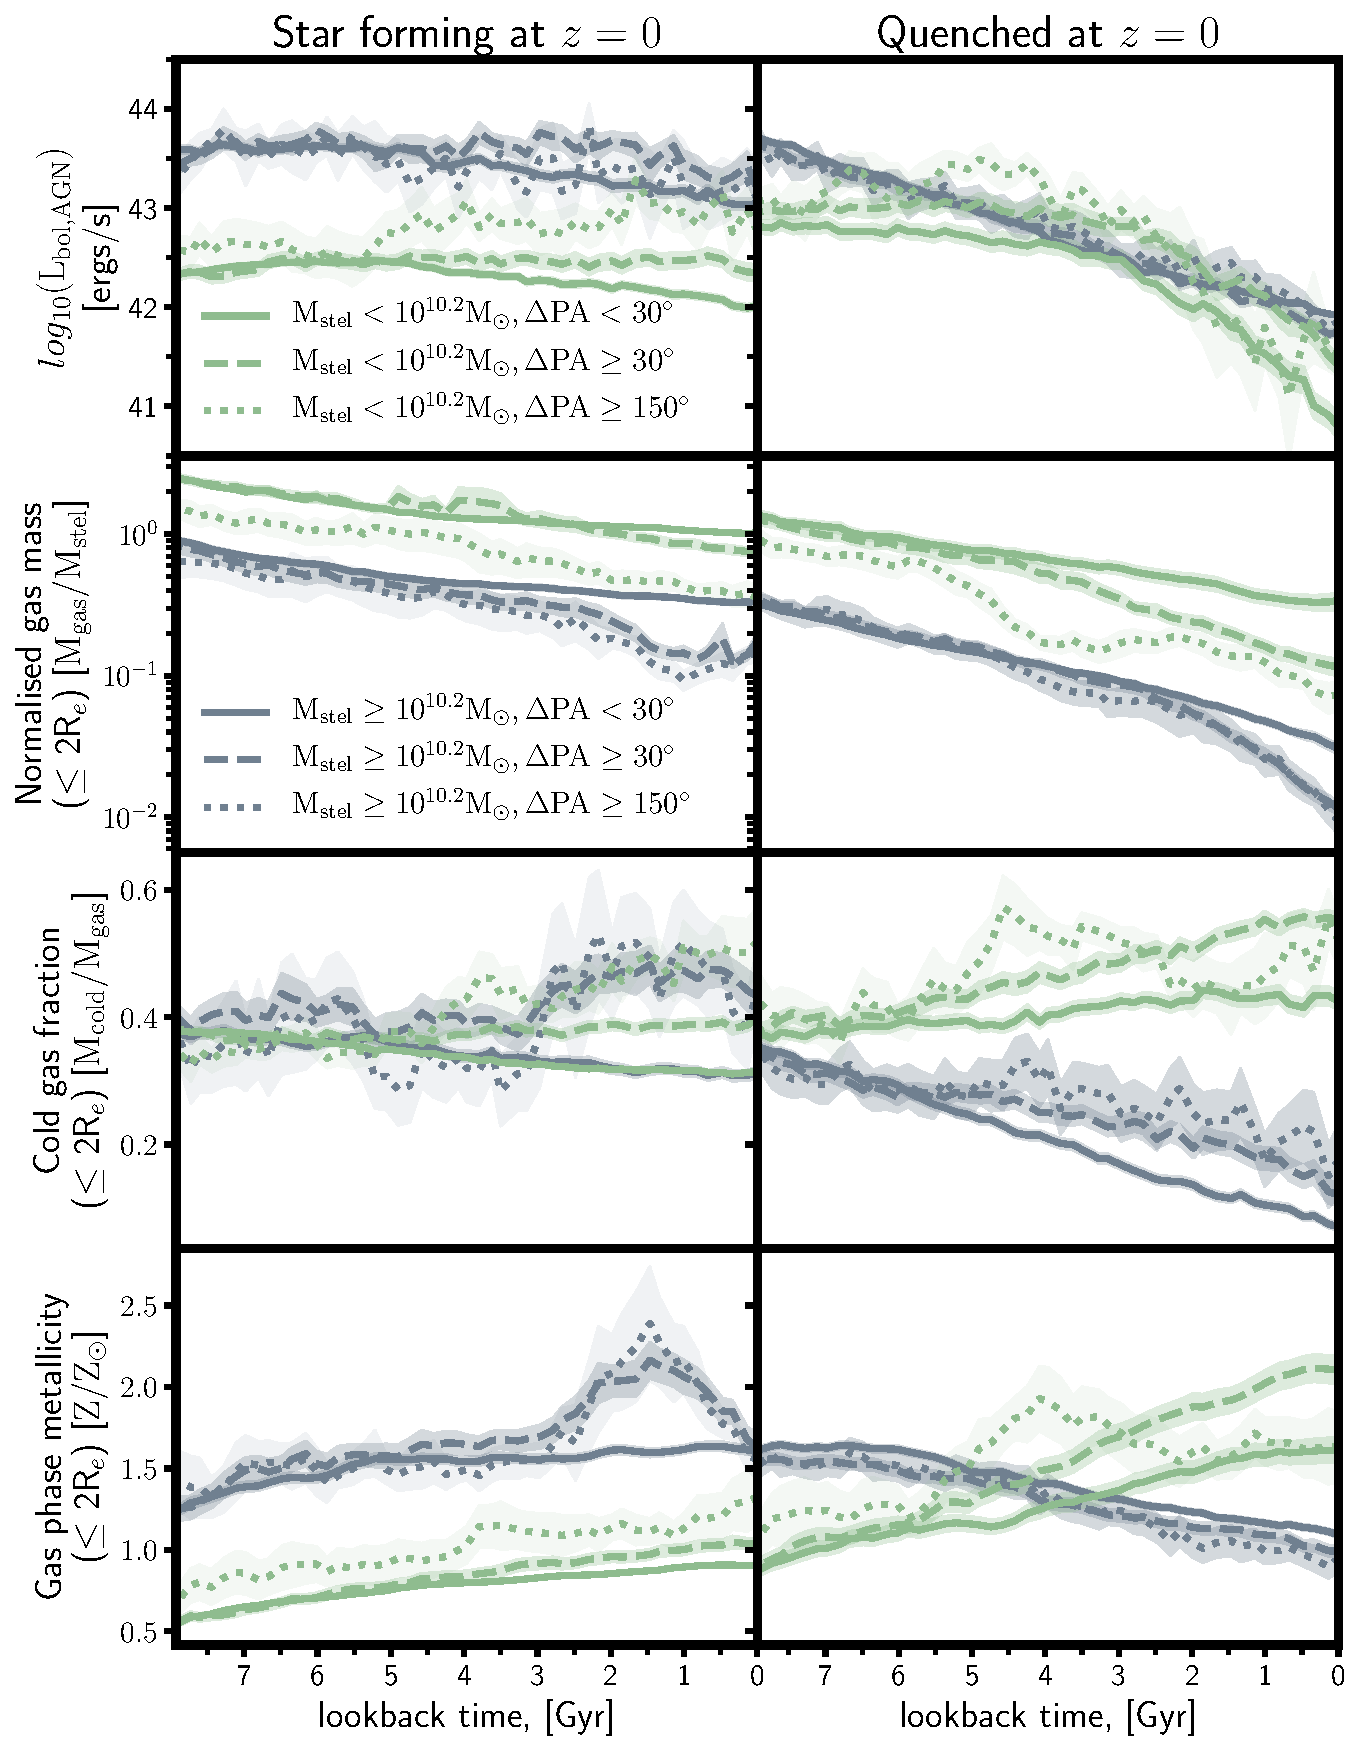
\includegraphics[width=\linewidth]{misalignment_BH/time_evo_letter_without_BH_props.pdf}
    \caption{Time evolution of (rows top to bottom) black hole luminosity ($\mathrm{log_{10}(L_{bol, AGN})}$), normalised gas mass ($\mathrm{M_{gas}/M_{stel}}$), cold and star forming gas fraction ($\mathrm{M_{cold}/M_{stel}}$), and, gas phase metallicity for star forming (left) and quenched galaxies (right) identified at $z=0$. Galaxies are divided into low mass (green; $\mathrm{M_{stel} < 10^{10.2}M_{\odot}}$) and high mass (grey; $\mathrm{M_{stel} > 10^{10.2}M_{\odot}}$) populations. Both are subdivided by misalignment ($\Delta$PA $< 30^{\circ}$: solid, $\geq 30^{\circ}$: dashed, and  $\geq 150^{\circ}$: dotted). Each line shows the mean for the population with the shaded region corresponding to the standard error.}
    \label{fig:overall_pop}
\end{figure}

\begin{figure}
	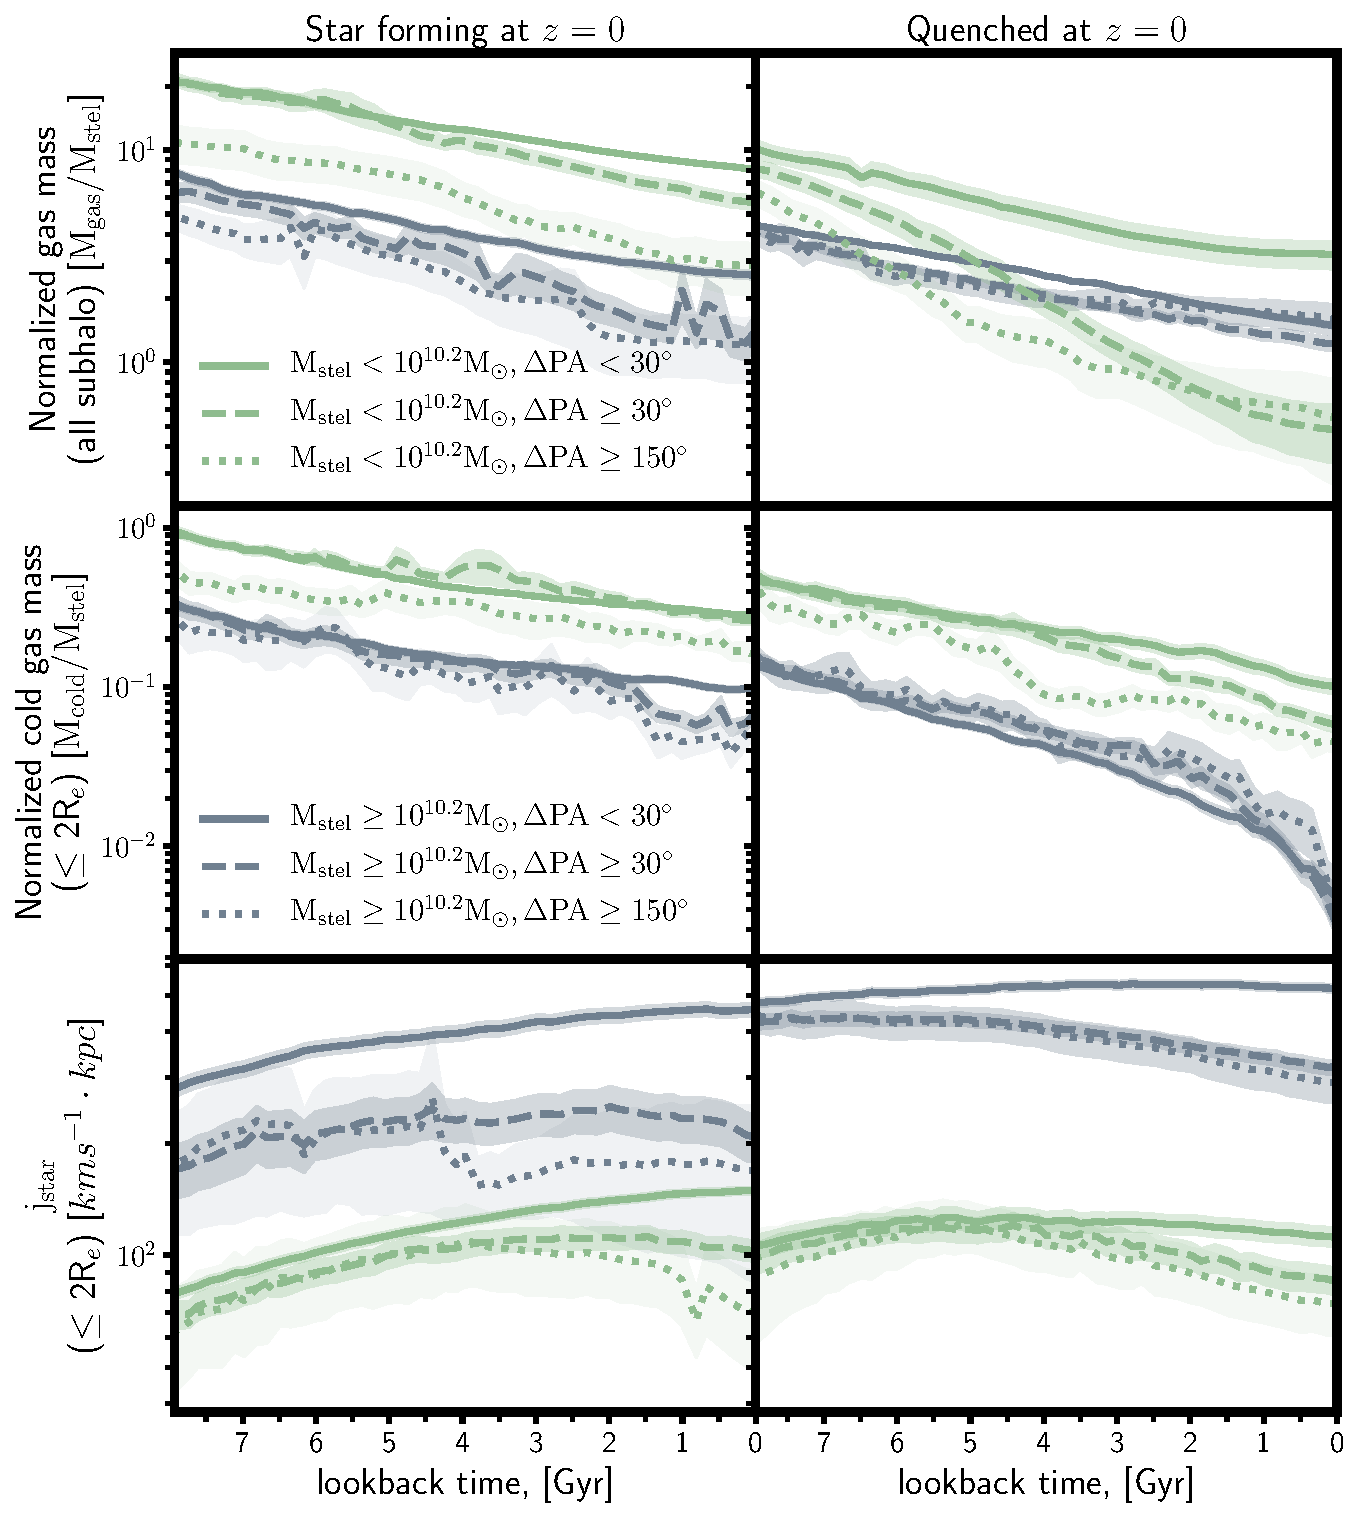
\includegraphics[width=\linewidth]{misalignment_BH/time_evo_supplement_no_feedback.pdf}
    \caption{Time evolution of (rows top to bottom) of normalized gas mass within the total subhalo ($\mathrm{M_{gas}/M_{stel}}$), normalized cold gas mass ($\mathrm{M_{cold}/M_{stel}}$) and specific stellar angular momentum ($\mathrm{j_{star}}$), for star forming (left) and quenched galaxies (right) identified at $z=0$. We show both low mass (green; $\mathrm{M_{stel} < 10^{10.2}M_{\odot}}$) and high mass (grey; $\mathrm{M_{stel} > 10^{10.2}M_{\odot}}$) galaxies. Both are subdivided by misalignment ($\Delta$PA $< 30^{\circ}$: solid, $\geq 30^{\circ}$: dashed, and  $\geq 150^{\circ}$: dotted). Each line shows the mean for the population with the shaded region corresponding to the standard error.}
    \label{fig:overall_pop_additional}
\end{figure}

\begin{sidewaystable}
\centering
\begin{tabular}{llllllll}
\hline
&  $\mathrm{L_{bol,AGN}}$ & $\mathrm{M_{gas} / M_{stel} (< 2R_e)}$ & $\mathrm{M_{cold} / M_{gas}}$ & $\mathrm{Z / Z_{\odot}}$ & $\mathrm{M_{gas}/M_{stel} (total)}$ & $\mathrm{M_{cold}/M_{stel}}$ & $\mathrm{j_{star}}$ \\
\hline
Low mass star forming & ++ & $--$ & ++ & + & $--$ & 0/$-$C & $--$ \\
High mass star forming & + & $-$/bump & ++/bump & ++/bump & $--$ & -/bump & $--$ \\
Low mass quenched & +/bumpC & $--$/bumpC & ++/bumpC & ++/bumpC & $--$ & $--$ & $--$ \\
High mass quenched & 0 & $-$ & ++ & 0$-$ & 0 & 0+ & $--$ \\
\end{tabular}
\caption{Truth table summarising the correlations found in Figure \ref{fig:overall_pop} between BH luminosity, normalised gas mass ($\mathrm{< 2R_e}$), cold gas fraction and gas phase metallicity (first four columns) with misalignment identified at $z=0$. The latter three columns additionally show the correlations found in the Supplementary material between total normalised gas mass (in subhalo), normalised cold gas mass and specific stellar angular momentum with misalignment. Correlations are shown individually for misaligned galaxies separated by both stellar mass and SFR at $z=0$. ++, + ($--$, $-$) refer to strong and mild positive (negative) correlations, 0 to no correlation and bump indicates a feature in the curve. A C is appended if the correlation/feature is only applicable to counter-rotating galaxies.}
\label{tab:truth}
\end{sidewaystable}

\subsection{Star forming galaxies}
In Figure \ref{fig:overall_pop}, misaligned (dashed) and counter-rotating (dotted) low mass star forming galaxies (green curves in left column) exhibit increased BH luminosity (top row; $\mathrm{log_{10}(L_{bol, AGN})}$) and a decreased total gas fraction within 2$\mathrm{R_{e}}$ (second row; $\mathrm{M_{gas} / M_{stel}}$) over the last 8 Gyr relative to those aligned (solid). In TNG, galaxies in this mass range almost exclusively exhibit quasar mode feedback, suggesting this mode's correlation with misalignment (as shown by both increased BH luminosity and potential outflows seen in a lowered gas fraction). Those misaligned also demonstrate positive correlations with the fraction of cold or star forming gas (third row; $\mathrm{M_{cold} / M_{gas}}$ where $\mathrm{M_{cold}}$ is selected by gas cells with $\mathrm{T < 10^{4.5}K}$ or SFR > 0) and gas phase metallicity (fourth row; $\mathrm{Z / Z_{\odot}}$) compared with the aligned. 
It is important to note that despite the increased fraction of cold or star forming gas for the misaligned galaxies, the overall gas mass is lower than the aligned. In particular, the higher gas metallicity for the misaligned galaxies could indicate accretion of pre-enriched or recycled material, or that fresh accretion is prevented by the radiative outflows. 
For each property, the misaligned population are consistent with the aligned prior to a look-back time of $\sim$5 Gyrs and diverge towards $z=0$.

High mass star forming galaxies (grey curves in left column) exhibit the same qualitative trends with misalignment as the low mass star forming galaxies, also showing positive correlations with BH luminosity, cold gas fraction and gas phase metallicity and a negative correlation with gas fraction (see also Table \ref{tab:truth}). Despite this, these trends are notably less linear (BH luminosity aside) with bumps seen at a look-back time at $\sim$1.5 Gyrs. As the total number of misaligned (counter-rotating) high mass star forming galaxies is 31 (8) we consider the bump, while significant, too dependent on a very small set of galaxies. The similarities between the low and high mass star forming galaxies could be indicative that they are subject to the same physical processes. 

\subsection{Quenched galaxies}
Quenched low mass galaxies (green curves in right column) also demonstrate positive correlations with BH luminosity, cold gas fraction and gas phase metallicity and a negative correlation with gas fraction. This appears to corroborate the possible relationship between misalignment and radiative feedback mode as seen for the star forming low mass galaxies. Trends of BH luminosity and gas fraction, however, are more prominent for the quenched galaxies (relative to the low mass star forming) and show deviations from the aligned galaxies at earlier look-back times. To understand this, we discuss the evolution of the black hole and related feedback in \S\ref{sec:evolution}.
 
Trends for the quenched high mass galaxies are generally less distinct. Despite this, the gas-phase metallicity is typically lower for those misaligned at $z=0$ in contrast to the three other sub-populations. In addition we find that despite a decreased gas fraction within 2$\mathrm{R_{e}}$, the misaligned galaxies show typically higher cold gas masses (within 2$\mathrm{R_{e}}$) and no overall decrease in gas mass (within the overall subhalo) relative to the aligned (supplementary material; rows one and two). This may indicate that for the high-mass quenched galaxies the accretion of pristine gas and gas rich minor mergers is important for decoupling their rotation. This could be a natural result of high-mass quenched galaxies hosting smaller gas reservoirs, meaning that a small amount of accretion onto the galaxy (relatively to late-types) is sufficient to cause misalignment. An alternate explanation could be that enriched gas is preferentially lost due to feedback or environment. %\red{A notable consistency across all sub-populations is a similar degree of disruption to the angular momentum content of the gas (supplementary material; third row).}
 
\subsection{Evolution of the black hole feedback} \label{sec:evolution}
In Figure \ref{fig:BH_props} we show the time evolution of the mass of the black hole and of its associated feedback: the amount of energy injected into the surrounding gas cells. Here, we plot the average residual difference ($\Delta$Energy injected$\mathrm{ = E_{Misaligned/Counter-rotating} - E_{Aligned}}$) of misaligned (dashed) and counter-rotating (dotted) galaxies with respect to the aligned galaxies (grey dashed line at the origin) for both the low mass (first two rows) and high mass galaxies (bottom two rows).

\begin{figure}
	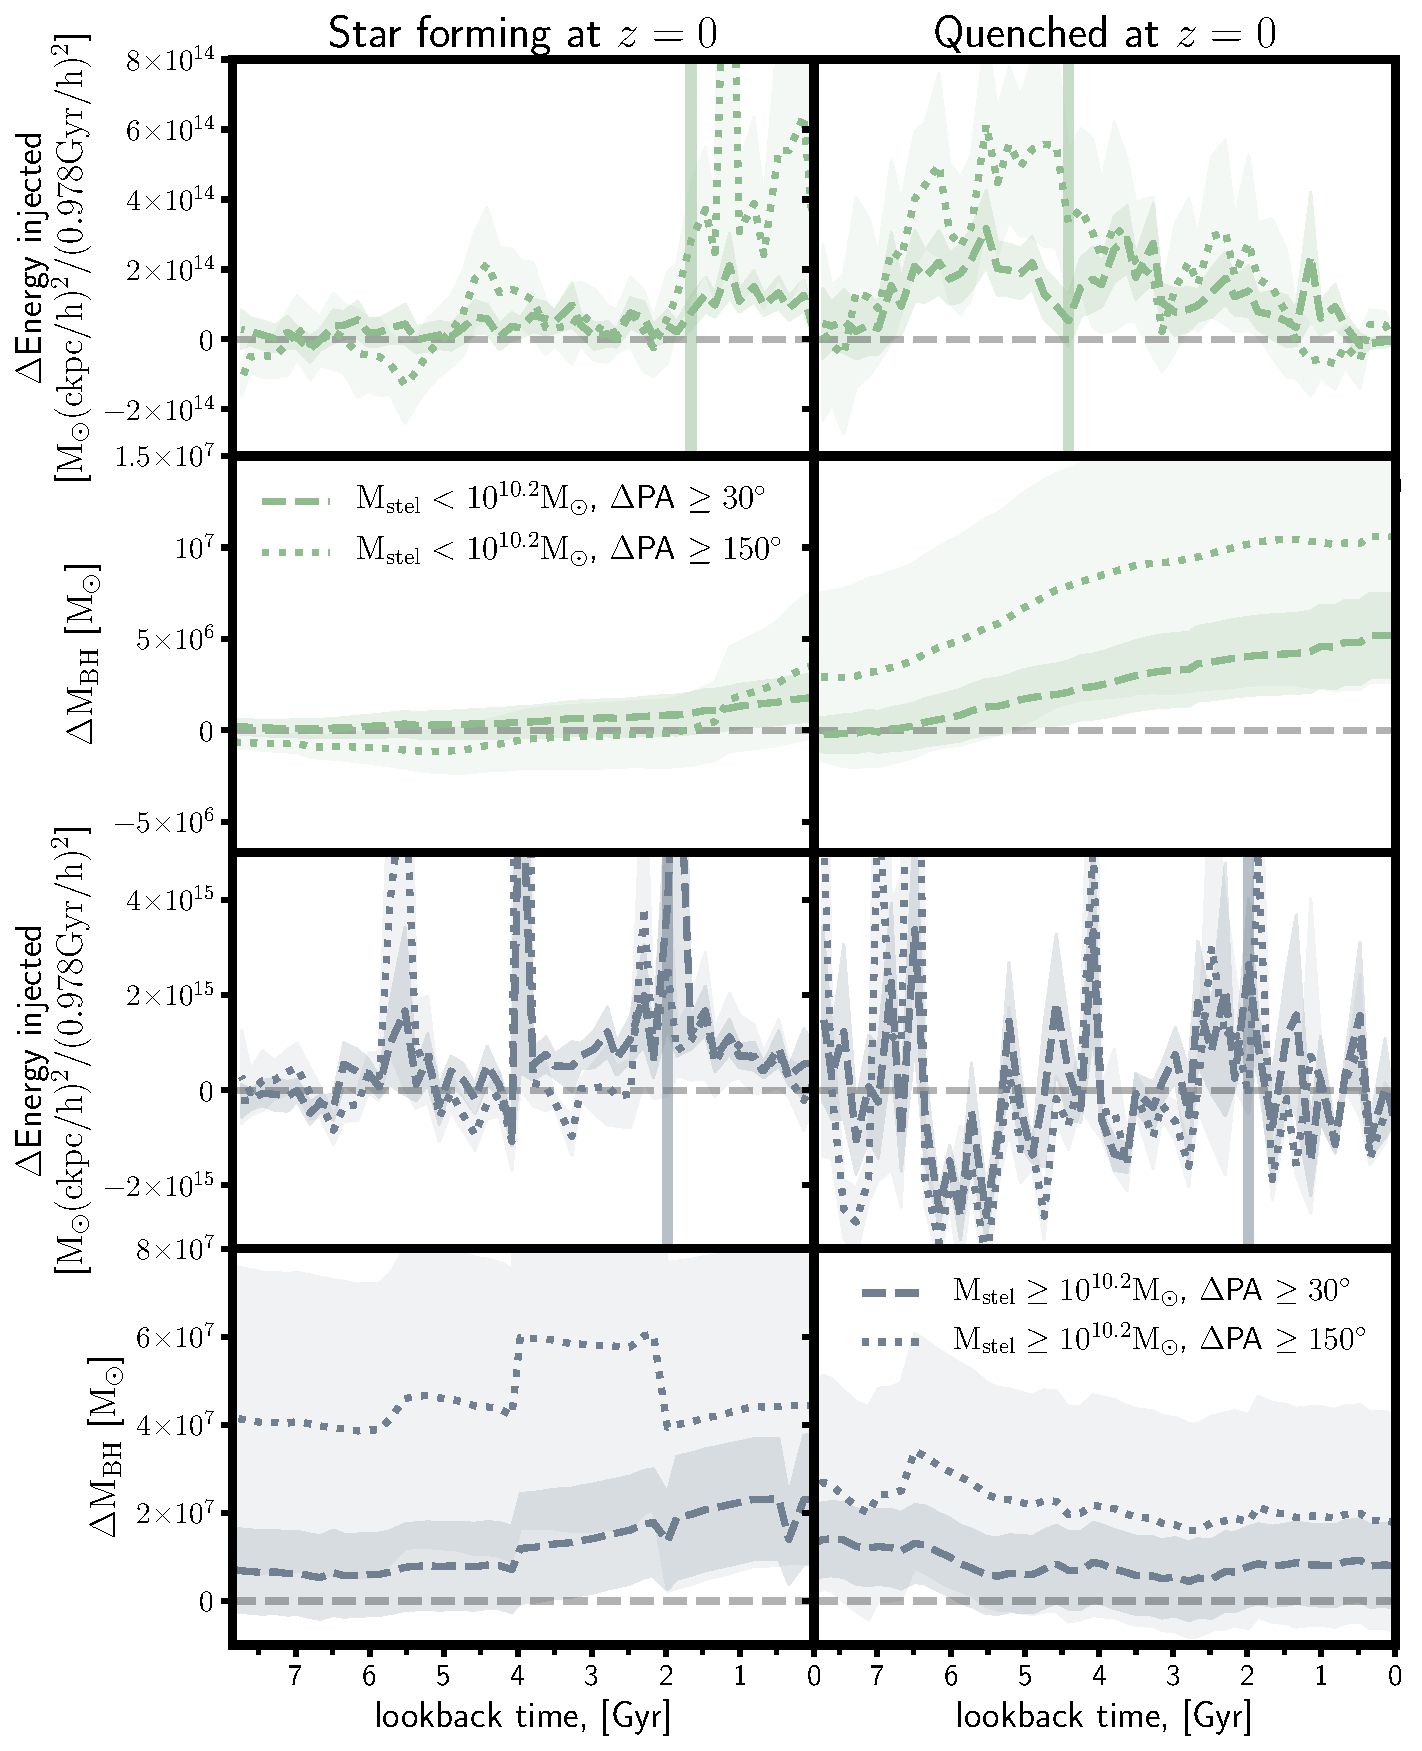
\includegraphics[width=\linewidth]{misalignment_BH/BH_props_only.pdf}
    \caption{Time evolution of black hole feedback energy injection and black hole mass for star forming (left) and quenched galaxies (right). Each row shows the residuals ($\Delta$Energy injected$\mathrm{ = E_{Misaligned/Counter-rotating} - E_{Aligned}}$) or $\Delta \mathrm{M_{BH}}$ where galaxies with $\Delta$PA $\geq 30^{\circ}$ (dashed) and $\Delta$PA $\geq 150^{\circ}$ (dotted) are defined relative to $\Delta$PA$ < 30^{\circ}$. The vertical line in the energy injection panels represents the time at which 50\% of the energy over the last 8 Gyrs has been injected. The top (bottom) two rows show the trends for low (high) mass galaxies.}
    \label{fig:BH_props}
\end{figure}

For the low mass galaxies, we find that the rate of energy injection is typically elevated for counter-rotating galaxies, however a clear boost can be seen for all those that are misaligned at $z=0$. The look-back time of peak energy injection is earlier for quenched galaxies relative to the star forming (the solid vertical line represents the time at which 50\% of the energy over the last 8 Gyrs has been injected). Misaligned star forming galaxies show far more recent feedback and BH luminosity, possibly indicative that the feedback has not fully suppressed star formation yet. Conversely, the quenched galaxies exhibit earlier peak energy injection which through this feedback suppressing star formation leads to the quenched classification at $z=0$. For this reason selecting misaligned star forming and quenched galaxies at $z=0$ will naturally lead to different time correlations in BH activity.

We also show the residual time evolution of black hole mass with respect to the aligned galaxies (Figure \ref{fig:BH_props} row 2 for low mass galaxies). We find that BH growth correlates with the time scales of energy injection, indicating the close relationship between feedback and accretion for those misaligned. The causality between BH growth and feedback is however not clear. While BH growth leads to increased feedback by design, with respect to a possible correlation between feedback and the onset of misalignment the question of causality remains. One possibility is that the angular momentum is disrupted prior to feedback, potentially due to mergers. Alternatively, gas removal due to feedback could facilitate (re-)accretion of (misaligned) gas which disrupts angular momentum and then leads to increased BH growth. We again note that misaligned high mass star forming galaxies (third row, left panel) demonstrate the same qualitative trends with BH feedback and growth as the low mass, corroborating that radiative feedback is likely dominant for this sub-sample. Misaligned and counter-rotating high mass quenched galaxies show little obvious trends of BH feedback energy and growth relative to the aligned.

\subsection{Correlating kinematic misalignment and AGN at $z=0$}
To understand how kinematic misalignment may correlate with BH luminosity at $z=0$ alone, in the top panel of Figure \ref{fig:PAdist}, we show the distribution of $\Delta$PA for the top 20\% BH luminosity in our low mass sample ($\mathrm{M_{stel} < 10^{10.2}M_{\odot}}$, both the star-forming and quenched galaxies) in comparison with a control sample (all defined at $z=0$). The control is made by taking the closest unique match in stellar mass for each high BH luminosity galaxy from the remainder of our sample. We find the two distributions are statistically indistinguishable (Anderson-Darling statistic; -0.001 with a p-value of 0.348). In the bottom panel we show the same but instead we select the top 20\% in peak BH luminosity (for each galaxy in our low mass sample) over the last 8 Gyrs. In this instance the AGN bright galaxies are distinctly more misaligned than the mass matched control (Anderson-Darling statistic; 13.793 with a p-value of $3 \times 10^{-5}$). 

\begin{figure}
    \centering
	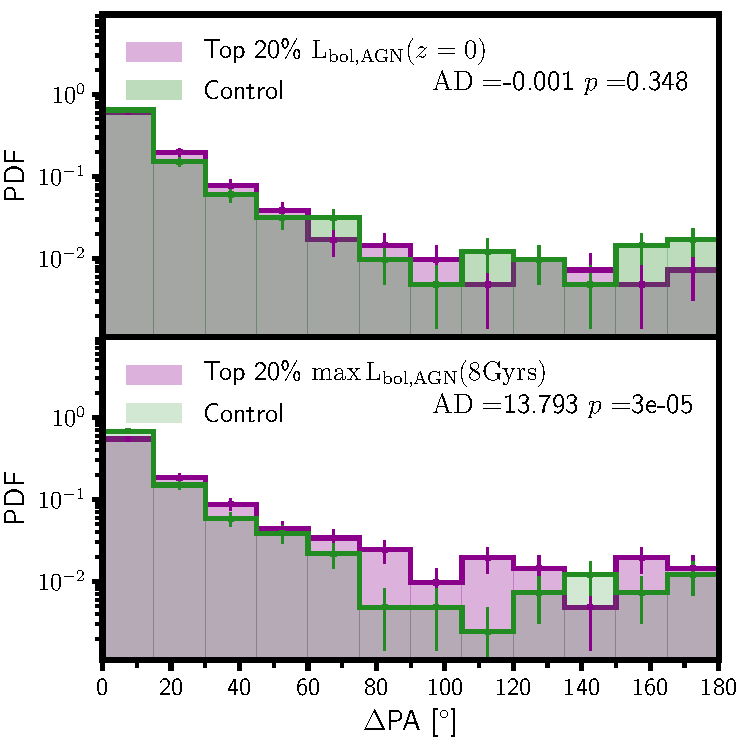
\includegraphics[width=0.9\linewidth]{misalignment_BH/PA_distribution_low_mass_z0_max_comparison.pdf}
    \caption{Probability density function of kinematic misalignment as defined by $\Delta$PA at $z=0$ for low mass galaxies ($\mathrm{M_{stel} < 10^{10.2}M_{\odot}}$). In both panels the brightest 20\% in $\mathrm{L_{bol,AGN}}$ (purple) compared with a mass matched control (green) is shown. The top panel shows the brightest in $\mathrm{L_{bol,AGN}}$ at $z=0$ only, whereas the bottom panel shows those with the brightest peak $\mathrm{L_{bol, AGN}}$ over the last 8 Gyrs. In each panel the Anderson-Darling statistic with a corresponding p-value is shown. We find no statistical difference between the active galaxies and the control for those selected at $z=0$ only, whereas we find that those which have been the most luminous over the last 8 Gyrs are distinctly more misaligned.}
    \label{fig:PAdist}
\end{figure}

This demonstrates that despite the inherent relationship between BH luminosity, feedback, and gas kinematics, considering the overall distribution of $\Delta$PA split on instantaneous luminosity at $z=0$ does not necessitate that correlation is found. This matches that of observations in MaNGA \citep[Figure 6 in][]{ilha2019}, who also find no correlation between active galaxies and a control sample. We emphasise that while our results indicate a correlation between feedback and misalignment, the decoupled rotation of gas can remain for several Gyr after initially becoming misaligned, meaning that a single epoch is unlikely to characterise the relationship for an ensemble of galaxies.

We note that IllustrisTNG typically under-produces bright AGN ($\mathrm{L_{X-ray}(2-10 keV) > 10^{44}ergs^{-1}}$) for $z \leq 1$ in contrast with observational constraints \citep[see][]{habouzit2019}. Given this and the uncertainty in estimating BH luminosity from simulations (treatment of radiatively efficient and inefficient AGN \& obscuration), we chose to select by percentile rather than cutting on absolute luminosity. Regardless, selecting only bright AGN in this way or choosing a higher percentile does not change our conclusions.

\section{Summary} \label{sec:summary_BH}
In this chapter, we study the relationship between BH luminosity, BH feedback and kinematic misalignment between stars and gas for galaxies in TNG100. We use mock observations of an IFS survey (MaNGA) built from galaxies in TNG100, to identify kinematic misalignment ($\Delta$PA; difference in PAs of stars and gas) at $z=0$. We split our mock IFS sample on stellar mass to separate the impact of `quasar' feedback from `kinetic' feedback. We follow the time evolution of BH luminosity and energy injection from BH feedback in leading up to misalignment (or counter-rotation) at $z=0$. We also compare the $z=0$ distributions of $\Delta$PA of the most luminous BHs in our sample against a control. Our conclusions are as follows.
\begin{enumerate}
    \item Low mass galaxies with misalignment (and counter-rotation) at $z=0$ typically have had boosted BH luminosity, BH growth, and significantly more energy injected into the gas over the last 8 Gyr in comparison to aligned galaxies. Gas is potentially blown out due to the AGN feedback, losing angular momentum towards $z=0$. Along with the feedback there is an increase in the fraction of cold phase gas within 2$\mathrm{R_{e}}$ (seen also for all high mass galaxies), along with an increased metallicity. These trends are seen for low mass star-forming and quenched galaxies, and high-mass star-forming galaxies split at $z=0$.
    
    \item The epoch of peak energy injection from the quasar mode feedback is different as a function of $z=0$ sSFR for misaligned low mass galaxies. This can be explained by the relationship between energy injection from feedback and galaxy quenching. Misaligned quenched galaxies have typically experienced peak energy injection from the BH at earlier times which has since acted to suppress star formation, whereas misaligned star forming galaxies exhibit more recent energy injection.

    \item Quenched high mass galaxies with misalignment (and counter-rotation) at $z=0$ typically have similar BH luminosity over the last 8 Gyr with respect to aligned galaxies and decreased gas mass is  seen within 2$\mathrm{R_{e}}$ (but not for all gas associated with the total subhalo). Gas phase metallicity is also lower with respect to aligned galaxies. This suggests that the origin of misalignment in massive quenched galaxies is more likely due to accretion of pristine gas or loss of enriched gas. 
    
    \item We find that the distributions of kinematic misalignment are statistically indistinguishable between the top 20\% in BH luminosity of low mass galaxies in our sample and a mass matched control at $z=0$. This matches observations \citep[see Figure 6 in][]{ilha2019}. Misalignment may initially occur at a similar time to the initial high accretion state (and hence peak BH luminosity), however misalignment can persist/correlate on much longer timescales. To test this we split by the top 20\% in maximum BH luminosity (for each galaxy) over the last 8 Gyrs in comparison with a control. We find that the most luminous AGN over the last 8 Gyrs are significantly more misaligned at $z=0$. This result suggests that while one may not expect correlation with misalignment when considering BH activity at $z=0$ alone, the relationship between BH luminosity and misalignment in low mass galaxies is clear. 
\end{enumerate}
While this work clearly demonstrates the correlation between BH activity and kinematic misalignment, it makes no comment on causality. Further work is required to understand what triggers the initial high accretion mode and following period of feedback for both low and high mass galaxies.
\red{expand on further work.}